\documentclass[a4paper, 10pt, ]{article}

\input{./COMMONFILES/preamble.tex}

% -----------------------------------------------------------------------------

\def\oznacenieCelku{Kolekcia učebných textov}

% -----------------------------------------------------------------------------


\def\KUTporadoveCislo{dev250819}

% \def\oznacenieVerzie{v0.9}
\def\oznacenieVerzie{\phantom{v1.0}}

\def\mesiacRok{august 2025}

\def\authorslabel{MT}






% -----------------------------------------------------------------------------

\begin{document}

% -----------------------------------------------------------------------------
% Uvodny nadpis

\noindent
\parbox[t][18mm][c]{0.3\textwidth}{%
\raisebox{-0.9\height}{%
\phantom{.}\includegraphics[height=18mm]{./COMMONFILES/URKFEIlogo.pdf}%
}%
}%
\parbox[t][18mm][c]{0.7\textwidth}{%
\raggedleft

\sffamily
\fontsize{16pt}{18pt}
\fontseries{sbc}
\selectfont

\noindent
\textcolor[rgb]{0.75, 0.75, 0.75}{\textls[25]{\oznacenieCelku}}
}%

\noindent
\parbox[t][16mm][b]{0.5\textwidth}{%
\raggedright

\color{Gray}
\sffamily

\fontsize{12pt}{12pt}
\selectfont
\mesiacRok

\fontsize{6pt}{10pt}
\selectfont
github.com/OkoliePracovnehoBodu/KUT

\fontsize{8pt}{10pt}
\selectfont
\authorslabel




}%
\parbox[t][16mm][b]{0.5\textwidth}{%
\raggedleft

\sffamily

\fontsize{6pt}{6pt}
\selectfont

\textcolor[rgb]{0.68, 0.68, 0.68}{\oznacenieVerzie}


\fontsize{14pt}{14pt}
\selectfont

\bfseries

\includegraphics[height=12pt]{./COMMONFILES/KUT_logo_v0.1.pdf}%
{%
\textls[-50]{\KUTporadoveCislo}
}%
}%

% -----------------------------------------------------------------------------




\vspace{6mm}

% ---------------------------------------------
\sffamily
\bfseries
\fontsize{18pt}{21pt}
\selectfont

\begin{flushleft}
    Laboratórne zariadenie LMOT:\\ orientačný prehľad
\end{flushleft}

\bigskip

% -----------------------------------------------------------------------------
\normalsize
\normalfont
% -----------------------------------------------------------------------------

\lstset{style=mystyle}










\noindent
\lettrine[lines=1, nindent=1pt, loversize=0.0]{C}{ieľom} 
textu je opis laboratórneho zariadenia LMOT predstavujúceho fyzický model spojitého dynamického systému..


\section{Opis dynamického systému}

LMOT je laboratórne zariadenie predstavujúce reálny dynamický systém. Pozostáva z malého jednosmerného motora, tachodynama, ktoré je na spoločnom hriadeli s~motorom, a z elektronických obvodov, ktoré zabezpečujú napájanie motora. Elektronickymi obvodmi sú tiež dané dominantné statické a dynamické vlastnosti výsledného systému. Do istej miery je možné tieto vlastnosti meniť manuálnym nastavením príslušného potenciometra.

Systém má jeden vstupný signál a jeden výstupný signál. Výstupný signál je priamo úmerný uhlovej rýchlosti jednosmerného motora, ktorá je snímaná tachodynamom. Vstupný signál ovláda napájanie motora.

Polohou potenciometra je v podstate daná prevádzková podmienka alebo prevádzkové nastavenie zariadenia. K~dispozícii je signál zodpovedajúci polohe potenciometra a teda tým je k dispozícii informácia o prevádzkovom nastavení systému.

LMOT (čítaj \emph{elmot}) je akronym pre „laboratórny motorček“, prípadne pre „little motor“.





\section{Rozsahy a jednotky signálov}

Z opisu predmetného dynamického systému vyplýva, že systém má jeden výstupný signál, jeden vstupný signál a manuálne nastaviteľnú prevádzkovú podmienku.

Vstupný a výstupný signál nadobúdajú hodnoty v~rozsahu $0$ až $10$ pričom ide o~napäťové signály vo voltoch [V].

Prevádzkové podmienka systému sa nastavuje manuálne otáčaním potenciometra. Signál o polohe potenciometra nadobúda hodnoty v rozsahu $0$ [V] až $10$ [V].





\begin{center}

\vspace{-10pt}    
    
\tabcaption{Rozsahy a jednotky signálov}
\label{tab:rozsahy_a_jednotky_signalu}

\lstyle

\begin{tabular*}{\textwidth}{@{ \extracolsep{\fill}} lll}
\toprule
Signál & Rozsah hodnôt & Jednotka \\
\midrule
Vstup & $0$ až $10$ & V (volt) \\
Výstup & $0$ až $10$ & V (volt) \\
Prevádzkové nastavenie & $0$ až $10$ & V (volt) \\
\bottomrule
\end{tabular*}


\end{center}







\section{Schematické znázornenie systému}


\begin{center}

    \vbox{%


        \makebox[\textwidth][c]{%
        
\includegraphics[width=1\textwidth,keepaspectratio]{LMOT_sch1.pdf}
        }

        \figcaption{ 
            Signály systému LMOT.
        }
        \label{LMOT_sch1}
    }%vbox

\end{center}


\begin{center}

    \vbox{%


        \makebox[\textwidth][c]{%
        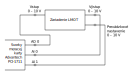
\includegraphics[width=1\textwidth,keepaspectratio]{LMOT_sch2.pdf}
        }

        \figcaption{ 
            Schéma pripojenia laboratórneho zariadenia k svorkám meracej karty Advantech PCI-1711, pričom AO~$0$ je analógový výstup meracej karty a~AI~$0$, AI~$1$ sú analógové vstupy meracej karty.
        }
        \label{LMOT_sch2}
    }%vbox

\end{center}



\section{Fotografie}

TODO:

\begin{itemize}
    \item Celkový pohľad na zariadenie
    \item Motor a tachodynamo
    \item Elektronické obvody zariadenia
    \item Predný panel so svorkami a potenciometrom
\end{itemize}







































































% -----------------------------------------------------------------------------

\end{document}

% -----------------------------------------------------------------------------